\documentclass[a4paper,
fontsize=11pt,
%headings=small,
oneside,
numbers=noperiodatend,
parskip=half-,
bibliography=totoc,
final
]{scrartcl}

\usepackage{synttree}
\usepackage{graphicx}
\setkeys{Gin}{width=.6\textwidth} %default pics size

\graphicspath{{./plots/}}
\usepackage[ngerman]{babel}
\usepackage[T1]{fontenc}
%\usepackage{amsmath}
\usepackage[utf8x]{inputenc}
\usepackage [hyphens]{url}
\usepackage{booktabs} 
\usepackage[left=2.4cm,right=2.4cm,top=2.3cm,bottom=2cm,headheight=25.60228pt,includeheadfoot]{geometry}
\usepackage{eurosym}
\usepackage{multirow}
\usepackage[ngerman]{varioref}
\setcapindent{1em}
\renewcommand{\labelitemi}{--}
\usepackage{paralist}
\usepackage{pdfpages}
\usepackage{lscape}
\usepackage{float}
\usepackage{acronym}
\usepackage{eurosym}
\usepackage[babel]{csquotes}
\usepackage{longtable,lscape}
\usepackage{mathpazo}
\usepackage[flushmargin,ragged]{footmisc} % left align footnote

%%url brekas grrr
\def\UrlBreaks{\do\a\do\b\do\c\do\d\do\e\do\f\do\g\do\h\do\i\do\j\do\k\do\l%
\do\m\do\n\do\o\do\p\do\q\do\r\do\s\do\t\do\u\do\v\do\w\do\x\do\y\do\z\do\0%
\do\1\do\2\do\3\do\4\do\5\do\6\do\7\do\8\do\9\do\-}%

\usepackage{listings}

\urlstyle{same}  % don't use monospace font for urls

\usepackage[fleqn]{amsmath}

%adjust fontsize for part

%% geometry
\clubpenalty = 10000 
\widowpenalty = 10000 
\displaywidowpenalty = 10000
%% tightlist

\providecommand{\tightlist}{%
  \setlength{\itemsep}{0pt}\setlength{\parskip}{0pt}}

\usepackage{sectsty}
\partfont{\large}

%Das BibTeX-Zeichen mit \BibTeX setzen:
\def\symbol#1{\char #1\relax}
\def\bsl{{\tt\symbol{'134}}}
\def\BibTeX{{\rm B\kern-.05em{\sc i\kern-.025em b}\kern-.08em
    T\kern-.1667em\lower.7ex\hbox{E}\kern-.125emX}}

\usepackage{fancyhdr}
\fancyhf{}
\pagestyle{fancyplain}
\fancyhead[R]{\thepage}

%meta

%meta

\fancyhead[L]{T. Bader \\ %author
LIBREAS. Library Ideas, 29 (2016). % journal, issue, volume.
\href{http://nbn-resolving.de/urn:nbn:de:kobv:11-100238925
}{urn:nbn:de:kobv:11-100238925}} % urn
\fancyhead[R]{\thepage} %page number
\fancyfoot[L] {\textit{Creative Commons BY 3.0}} %licence
\fancyfoot[R] {\textit{ISSN: 1860-7950}}

\title{\LARGE{Open-Access-Repositorien in der Schweiz und Österreich -- Auswertung des \textit{2014 Census on Open Access Repositories}}} %title %title
\author{Tabea Bader} %author

\setcounter{page}{}

\usepackage[colorlinks, linkcolor=black,citecolor=black, urlcolor=blue,
breaklinks= true]{hyperref}

\date{}
\begin{document}

\maketitle
\thispagestyle{fancyplain} 

%abstracts
\begin{abstract}
\small
Open-Access-Repositorien und werden in der wissenschaftlichen
Kommunikation immer wichtiger. Der ``2014 Census on Open Access
Repositories in Germany, Austria and Switzerland'' (Census 2014)
beschäftigte sich mit der Landschaft der Open-Access-Repositorien (OAR)
in den drei deutschsprachigen Ländern. In Bezug auf Deutschland wurden
die Daten bereits umfassend ausgewertet. Dieser Artikel gibt einen
Überblick über die Situation der Open-Access-Repositorien in der Schweiz
und Österreich auf Basis des Census 2014. Die Daten des Census werden
anhand der Kriterien Größe, Metadatenqualität, verwendete Software,
Rolle der Berliner Erklärung, Langzeitarchivierung,
Lizenzierungsmöglichkeiten unter anderem analysiert.

Bei den Auswertungen zeigte sich beispielsweise, dass Österreich und die
Schweiz wenige, aber dafür vergleichsweise große OAR haben. Die meisten
OAR verteilen sich auf Universitäten und außeruniversitäre
Forschungseinrichtungen. Fachhochschulrepositorien gibt es kaum, obwohl
es in beiden Ländern in etwa so viele Fachhochschulen wie Universitäten
gibt. Die Konformität der Metadaten mit den Vorgaben des
DINI-Zertifikats 2010 ist eher gering, jedoch muss beachtet werden, dass
kein OAR in den Alpenstaaten überhaupt ein Zertifikat besitzt. Weiterhin
lässt sich festhalten, dass die Software-Lösung EPrints dominiert.

\begin{center}\rule{0.5\linewidth}{\linethickness}\end{center}

Open access repositories become more and more important in scholarly
research. The ``2014 Census on Open Access Repositories in Germany,
Austria and Switzerland'' investigated the landscape of Open Access
Repositories (OAR) in the three German speaking countries. In relation
to Germany the data has been analyzed already. This article gives an
overview of the situation of Open Access Repositories in Switzerland and
Austria.

The Census data are surveyed regarding the criteria size, metadata
quality, software used, the role of the Berlin Declaration, long term
archiving, licensing options and others.

The findings were amongst others that Austria and Switzerland have few
but big repositories. Most OAR are connected to universities and
non-university research institutions. Repositories at universities of
applied sciences are nearly non-existent although there are almost as
much universities of applied sciences as there are universities in both
countries. Conformity with the DINI metadata standards is low, but one
has to keep in mind that no OAR of the alpine states has a
DINI-certificate. Furthermore the analysis shows that the software
EPrints dominates.
\end{abstract}

%body
\textbf{Vorbemerkung der Redaktion: Dieser Beitrag basiert auf der
Nachnutzung von veröffentlichten Forschungsdaten durch Studierende in
einem Hauptseminar im Sommer 2015 am IBI der HU Berlin. Der Artikel ist
exemplarisch für eine Beitragsform, von der die LIBREAS-Redaktion
perspektivisch gerne viel mehr integrieren würde, um den bibliotheks-
und informationswissenschaftlichen Nachwuchs an das Publizieren
heranzuführen. Wir bitten die AutorIn und die LeserInnen an dieser
Stelle um Nachsicht, dass die Publikation des Beitrags erst in dieser
auf die Jubiläumsausgabe in 2015 folgenden LIBREAS-Ausgabe möglich war
und das verwendete Datenmaterial aus 2014 somit bereits zwei Jahre alt
ist. Weitere Analysen des Zahlenmaterials und ergänzende Erhebungen sind
ausdrücklich erwünscht.}

\section*{1 Einführung}\label{einfuxfchrung}

Dieser Artikel wertet den \enquote{2014 Census on Open Access
Repositories in Germany, Austria and Switzerland} (2014 Census) auf
Ergebnisse hinsichtlich der Alpenländer Österreich und Schweiz aus. Er
orientiert sich dabei an dem von Maxi Kindling und Paul
Vierkant\footnote{Vierkant, Paul; Maxi Kindling: Welche Institutionen
  betreiben Open-Access-Repositorien in Deutschland?. LIBREAS. Library
  Ideas, 26 (2014). http://libreas.eu/ausgabe26/07vierkantkindling/}
veröffentlichten Artikel über die deutschen Open-Access-Repositorien
(OAR), dem Open Access Repository Ranking (OARR)\footnote{\url{http://repositoryranking.org/},
  28.06.2016.} von 2014\footnote{Kindling, Maxi: Auswertungen und
  Forschungsdaten zum \enquote{2014 Census on Open Access Repositories
  in Germany, Austria and Switzerland}.
  \url{https://oanetzwerk.wordpress.com/2015/09/07/forschungsdaten-und-auswertungen-zum-2014-census-on-open-access-repositories-in-germany-austria-and-switzerland/},
  18.10.2015}. Eine Hausarbeit, die im Frühjahr 2015 für ein Seminar bei
Ulla Wimmer am Institut für Bibliotheks- und Informationswissenschaft
der Humboldt-Universität zu Berlin entstand, bildet die Grundlage des
Textes.

Der 2014 Census wurde im Zuge eines Projektseminars am Institut für
Bibliotheks- und Informationswissenschaft der Humboldt-Universität zu
Berlin erstellt, um einen Überblick über die Landschaft der
Open-Access-Repositorien (OAR) in deutschsprachigen Ländern zu
erhalten.\footnote{Vierkant, Paul; Maxi Kindling u.a.: Dataset Open
  access

  Research Data of the 2014 Census of Open Access Repositories in
  Germany, Austria and Switzerland.
  \url{http://www.zenodo.org/record/10734?ln=en/\#.VK/_3knvpWXc},
  26.02.2015.} Er \enquote{{[}\ldots{}{]} basiert auf einer qualitativen
Inhaltsanalyse der Webseiten der Repositorien, einer automatisierten
Validierung der über das OAI-PMH ausgelieferten Metadaten sowie einer
Umfrage unter Repositorienbetreibern}\footnote{Vierkant P., M. Kindling:
  Welche Institutionen betreiben Open-Access-Repositorien in
  Deutschland?.}.

Für die Auswahl der zu untersuchenden OAR wurde für den Census die
nachfolgende Definition verwendet:

\begin{quote}
\enquote{Open-Access-Repositorien sind für den Zweck dieser Studie
institutionelle und disziplinäre Repositorien aus Deutschland,
Österreich und der Schweiz, die mehrheitlich wissenschaftliche
Open-Access-Volltextveröffentlichungen vorhalten. Die
Volltextveröffentlichungen sind durch Metadaten beschrieben, die über
eine Weboberfläche (Such- und Browsefunktionalität) recherchierbar sind.
Die Open-Access-Repositorien sind mit einer funktionierenden Base-URL
für das OAI-PMH Harvesting bei Bielefeld Academic Search Engine (BASE)
registriert. Digitale Sammlungen, Forschungsdatenrepositorien, sowie
Open-Access-Repositorien von Verlagen, University Presses und
kommerzielle Dienste sind ausgeschlossen.}\footnote{Vierkant, P.; M.
  Kindling: Welche Institutionen betreiben Open-Access-Repositorien in
  Deutschland?.}
\end{quote}

Der Betrachtungsgegenstand setzt sich demzufolge aus den in BASE
registrierten OAR der beiden Länder zusammen, die von Universitäten,
Fachhochschulen und außeruniversitären Institutionen unterhalten werden.
Welche dazu gehören, wurde durch die Typisierungslisten der BMWF (heute
BMWFW) für Österreich und CRUS (heute swissuniversities) für die Schweiz
auf Grundlage der Zahlen von 2014 ermittelt.\footnote{\enquote{Der
  Erhebungszeitraum begann am 6. Januar 2014 und endete am 31. Januar
  2014.} Vierkant, P.; M. Kindling: Welche Institutionen betreiben
  Open-Access-Repositorien in Deutschland?.} Zum Untersuchungszeitraum
zählte die Studie 16 solcher Repositorien in der Schweiz und fünf in
Österreich. Laut der OpenDOAR-Liste der Länder besitzt die Schweiz 2016
17 und Österreich 22 OAR.\footnote{\url{http://www.opendoar.org/find.php?search=\&clID=\&ctID=\&rtID=\&cID=205\&lID=\&rSoftWareName=\&submit=Search\&format=summary\&step=20\&sort=r.rName\&rID=\&ctrl=new\&p=1};
  \url{http://www.opendoar.org/find.php?search=\&clID=\&ctID=\&rtID=\&cID=15\&lID=\&rSoftWareName=\&submit=Search\&format=summary\&step=20\&sort=r.rName\&rID=\&ctrl=new\&p=1},
  04.01.2016.} Dies kann darauf zurückzuführen sein, dass einige in
OpenDOAR gelistete Repositorien entsprechend der Definition für OAR
dieser Studie nicht berücksichtigt wurden oder 2014 noch nicht
existierten.

Da für Österreich und die Schweiz eine überschaubare Menge an OAR
vorzufinden sind, ist eine Aufteilung in Bundesländer bzw. Kantone, wie
es in der Auswertung für Deutschland geschehen ist, nicht überall
notwendig. Zudem finden sich in beiden Ländern nur institutionelle
Repositorien. Eine Differenzierung in disziplinäre und institutionelle
erfolgt demzufolge nicht.

\section*{2 Standorte}\label{standorte}

\paragraph{2.1 Schweiz}\label{schweiz}

Um zu Beginn einen Überblick über die Repositorien in der Schweiz zu
erhalten, wird zunächst betrachtet, wo sich diese befinden.

Die Schweiz hat 26 Kantone, für acht davon, d.h. weniger als ein
Drittel, sind OAR erfasst. Jedoch muss beachtet werden, dass in elf
Kantonen keine den Kriterien des Census entsprechende Hochschule
existiert, die ein Repositorium betreiben könnte.

\begin{figure}[htbp]
\centering
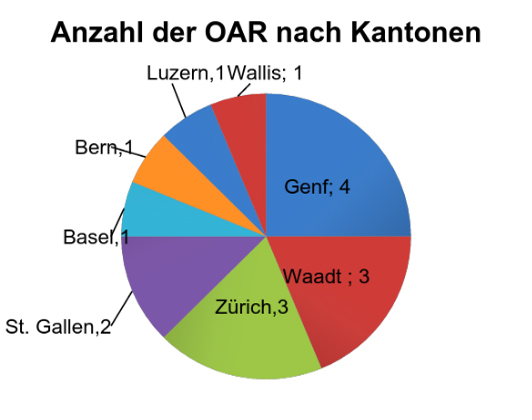
\includegraphics{img/abb1_anzahl_oar_kantone.jpg}
\caption{Schweiz nach Kantonen}
\end{figure}

Abbildung 1 zeigt, dass Genf mit vier OAR auf Kantonebene Vorreiter ist.
Eine Ursache dafür ist die renommierte Forschungseinrichtung der Physik,
die Europäische Organisation für Kernforschung (CERN), die dort ihren
Sitz hat und mit zwei OAR im Census 2014 vertreten ist. Auch in Waadt,
einer der beiden Kantone mit den zweitmeisten OAR, befinden sich an der
Ecole Polytechnique Fédérale de Lausanne zwei Repositorien.

Die Schweizer Kantone sind wie bereits erwähnt nicht gleichmäßig mit
Hochschulen ausgestattet, was zur Folge hat, dass nicht überall
akademische Repositorien angesiedelt sein können. Insgesamt verfügt die
Schweiz über 12 anerkannte universitäre Hochschulen und neun
Fachhochschulen. Die Fachhochschulen sind aus einem Verbund von
regionalen Hochschulen zusammengesetzt, die sich an verschiedenen
Standorten über die Kantone verteilt befinden und theoretisch, wie die
Hochschule für Technik Rapperswil, je ein eigenes Repositorium betreiben
könnten.

Mit 14 Hochschulen (zwei universitären Einrichtungen und zwölf
Fachhochschulen), besitzt der französischsprachige Kanton Waadt die
meisten. Darauf folgen das Tessin, Basel-Stadt, Genf und Luzern. Genf,
der Kanton mit den meisten Repositorien, unterhält sieben nicht
universitäre Hochschulen und eine Universität, während Zürich zwei
universitäre Hochschulen und drei Fachhochschulen aufweist und dabei
drei Repositorien unterhält, die alle drei an den universitären
Hochschulen angesiedelt sind.

Keine den Census-Kriterien entsprechenden Hochschulen und ebenfalls
keine Repositorien weisen die zehn Kantone Uri, Schwyz, Zug, Obwalden,
Nidwalden, Glarus, Appenzell-Ausserr- und Innerrhoden, Schaffhausen und
Thurgau auf. Der einzige italienischsprachige Kanton in der Schweiz, das
Tessin, besitzt zwar eine Universität, die USI Università della Svizzera
italiana und sechs Fachhochschulen, betreibt aber kein OAR.\footnote{Aus
  Informationen der Seite
  \url{http://www.swissuniversities.ch/de/hochschulraum/anerkannte-schweizer-hochschulen/}
  recherchiert.}

\paragraph{2.2 Österreich}\label{uxf6sterreich}

Im Census 2014 sind fünf österreichische Repositorien gelistet. Diese
befinden sich ausschließlich in der Hauptstadt Wien, die gleichzeitig
eines der neun Bundesländer darstellt.

Im bei der Datenanalyse vergleichend herangezogenen OARR 2015 sind mit
Tirol und der Steiermark mit je einem OAR auch weitere Bundesländer
Österreichs vertreten.

\section*{3 Institutionstypen}\label{institutionstypen}

\paragraph{3.1 Schweiz}\label{schweiz-1}

Das Feld der Institutionstypen teilt sich in der Studie auf
Universitäten, Fachhochschulen und außeruniversitäre
Forschungseinrichtungen auf. Abbildung 2 veranschaulicht, dass in der
Schweiz jeder dieser Typen als OAR-besitzende Institution vorkommt.
Dabei nehmen die Universitäten mit zehn von 16 Repositorien eine
deutliche Führungsrolle ein, während es mit der HSR Hochschule für
Technik Rapperswil nur eine einzige Fachhochschule gibt, die ein OAR
unterhält.\footnote{Eine auf Kantonebene aufgegliederte Auswertung kann
  bei der Autorin angefordert werden.} Wie groß ist nun der Anteil der
Institutionen, die in der Schweiz überhaupt ein OAR betreiben? In dieser
Auswertung werden keine außeruniversitären Forschungseinrichtungen
aufgeführt, da zur Gesamtzahl solcher Einrichtungen in der Schweiz keine
Daten ermittelt werden konnten.

\begin{figure}[htbp]
\centering
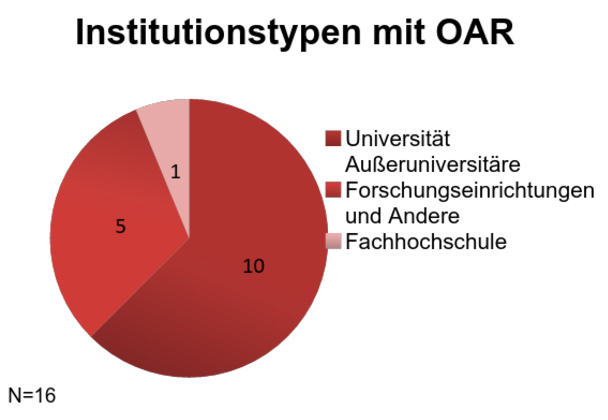
\includegraphics{img/abb2_institutionentypen_oar.jpg}
\caption{Schweiz - Institutstypen mit OAR}
\end{figure}

Laut CRUS (dem Vorgänger des gemeinsamen hochschulpolitischen Organs der
Schweiz \enquote{swissuniversities}) gab es 2014 21 Universitäten und
Fachhochschulen bzw. Fachhochschulverbünde in der Schweiz. Von diesen
besitzen neun ein OAR. Acht der zwölf Universitäten und nur eine der
insgesamt neun Fachhochschulverbünde haben ein Repositorium. An zwei
Universitäten werden jeweils zwei OAR betrieben, weswegen sich die
Anzahl der Universitäten mit Repositorium von zehn auf acht reduziert.
Abbildung 3 zeigt, dass nicht ganz die Hälfte aller
Hochschuleinrichtungen ein OAR betreiben, jedoch nur vier Schweizer
Universitäten kein Repositorium haben.

\begin{figure}[htbp]
\centering
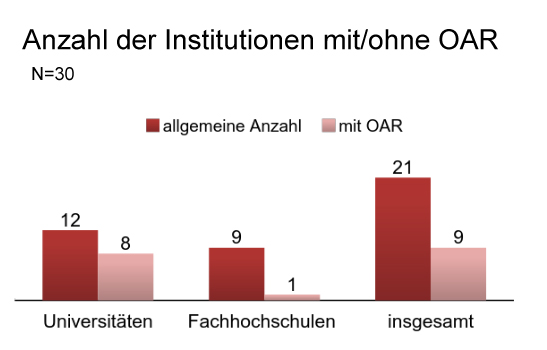
\includegraphics{img/abb3_institutionen_ch_oar.jpg}
\caption{Schweiz - Anzahl der Institutionen mit/ohne OAR}
\end{figure}

\paragraph{3.2 Österreich}\label{uxf6sterreich-1}

Wie in Abbildung 4 zu erkennen, betreiben in Österreich hauptsächlich
Universitäten OAR. Einzig die Österreichische Akademie der
Wissenschaften ist als nicht-universitäre Institution im Census
2014verzeichnet.

Wie groß ist die Anzahl der Institutionen, die in Österreich überhaupt
ein OAR betreiben?

Laut dem BMWF hatte Österreich 2014 22 Universitäten.\footnote{2015
  gelten die gleichen Zahlen. Gesamtübersicht Universitäten:
  \url{http://wissenschaft.bmwfw.gv.at/bmwfw/wissenschaft-hochschulen/universitaeten/gesamtuebersicht-universitaeten/},
  24.10.2015.} Von diesen sind im Census 2014 vier vertreten. Keine der
21 Fachhochschulen betreibt ein OAR. Das bedeutet, dass insgesamt nur
vier von 43 Hochschulen ein für den Census 2014 relevantes Repositorium
betreiben. Diese sehr geringe Anzahl überrascht. Es lässt sich jedoch
festhalten, dass es durchaus mehr Repositorien geben könnte, die nur
durch die Census-spezifische Definition nicht erfasst wurden.

\section*{4 Größe der OAR}\label{gruxf6uxdfe-der-oar}

Als Größe eines OAR wird die Anzahl der über die OAI-Schnittstelle
ausgelieferten Items in einem Repositorium definiert. Der Census 2014
kategorisiert Repositorien folgendermaßen nach ihrem Umfang: Kleine
Repositorien halten ein bis 1.000 Items vor, mittelgroße 1.001 bis 5.000
Items und als groß werden OAR bezeichnet, die 5.001 oder mehr Items
besitzen.\footnote{Vierkant, Paul: Eine kurze Geschichte der
  Open-Access-Repositorien-Landschaft in Deutschland von 1991-2013.
  Fußnote 7.
  \url{https://libreas.wordpress.com/2014/12/01/eine-kurze-geschichte-der-open-access-repositorien-landschaft-in-deutschland-von-1991-2013/},
  25.10.2015.}

\begin{figure}[htbp]
\centering
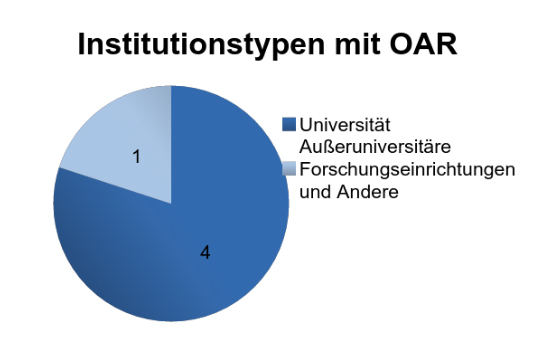
\includegraphics{img/abb4_institutionentypen_oar.jpg}
\caption{Österreich - Institutionstypen mit OAR}
\end{figure}

Die Mehrheit der Schweizer Repositorien sind groß. Kleine und mittlere
Repositorien gibt es zusammengenommen nur fünf.

In Österreich gibt es kein der Kategorisierung zufolge als klein
einzustufendes OAR. Es gibt drei mittelgroße und zwei große
Repositorien.

\begin{figure}[htbp]
\centering
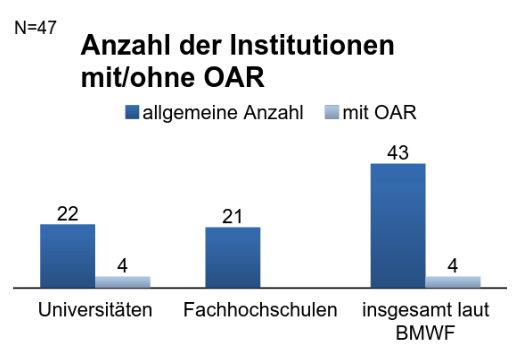
\includegraphics{img/abb5_institutionen_oar_at.jpg}
\caption{Österreich - Anzahl der Institutionen mit/ohne
OAR}
\end{figure}

\paragraph{Größe der OAR nach Institutionstyp --
Schweiz}\label{gruxf6uxdfe-der-oar-nach-institutionstyp-schweiz}

Insgesamt besitzen die OAR in der Schweiz 1.190.965 Items. Die meisten,
und zwar 706.526, verteilen sich auf Universitäts-OAR, während nur ein
Fachhochschul-OAR mit lediglich 314 Objekten in St.Gallen vorhanden ist.
Die außeruniversitären Forschungseinrichtungen hingegen halten mit
484.125 Items eine weitere große Menge vor. Sie haben einen hohen Anteil
an den gesamten Items in den Repositorien der Schweiz, obwohl es gerade
einmal fünf ihres Typs gibt. Der außeruniversitäre \emph{CERN Document
Server} ist mit 455.394 Items das größte OAR der Schweiz.

\begin{figure}[htbp]
\centering
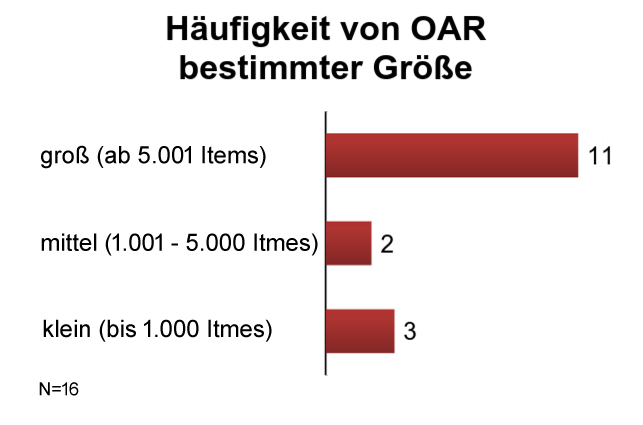
\includegraphics{img/abb6_oar_haeufigkeit.jpg}
\caption{Schweiz - Häufigkeit von OAR bestimmter Größe}
\end{figure}

Insgesamt werden in den Repositorien Österreichs 69.612 Items zur
Verfügung gestellt. Das größte Repositorium Österreichs wird von der
Österreichischen Akademie der Wissenschaften betrieben. Dort befinden
sich mehr als die Hälfte aller Items. Darauf folgen die drei OAR der
Universität Wien, wobei der Hochschulschriften-Service mit 23.947 Items
das größte ist. Das kleinste OAR ist das der Wirtschaftsuniversität
Wien, welches nur 2\% der Gesamt-Items ausmacht.

\begin{figure}[htbp]
\centering
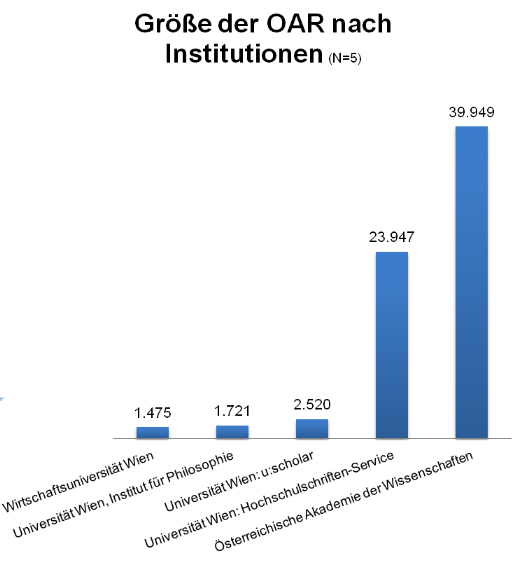
\includegraphics{img/abb7_groesse_oar_at.jpg}
\caption{Österreich - Größe der OAR nach Institutionen}
\end{figure}

\paragraph{Wachstum der OAR}\label{wachstum-der-oar}

Anhand der im Zeitraum vom 6. Januar 2013 bis zum 6. Januar 2014 zu den
einzelnen OAR hinzugefügten Items, lassen sich das prozentuale Wachstum
der verschiedenen Repositorien für diesen Zeitraum ermitteln.

Das stärkste Wachstum verzeichnet laut Tabelle 1 der \emph{CERN Document
Server} mit 381,98\%. Das sehr viel kleinere \emph{OpenAIRE Orphan
Record Repository} vergrößerte seine Item-Anzahl im Verhältnis am
zweitmeisten und konnte um rund 101\% wachsen. Auch dieses Repositorium
wird am CERN betrieben.

\begin{longtable}[c]{@{}lrrrr@{}}
\caption{Schweiz - Wachstum der OAR}\tabularnewline
\toprule
\begin{minipage}[b]{0.25\columnwidth}\raggedright\strut
OAR (N=16)
\strut\end{minipage} &
\begin{minipage}[b]{0.16\columnwidth}\raggedleft\strut
Anzahl Items 06.01.2013
\strut\end{minipage} &
\begin{minipage}[b]{0.16\columnwidth}\raggedleft\strut
Anzahl Items 06.01.2014
\strut\end{minipage} &
\begin{minipage}[b]{0.14\columnwidth}\raggedleft\strut
Absoluter Zuwachs von Items im Zeitraum 2013/14
\strut\end{minipage} &
\begin{minipage}[b]{0.14\columnwidth}\raggedleft\strut
Zuwachs von Items im Zeitraum 2013/14 in Prozent
\strut\end{minipage}\tabularnewline
\midrule
\endfirsthead
\toprule
\begin{minipage}[b]{0.25\columnwidth}\raggedright\strut
OAR (N=16)
\strut\end{minipage} &
\begin{minipage}[b]{0.16\columnwidth}\raggedleft\strut
Anzahl Items 06.01.2013
\strut\end{minipage} &
\begin{minipage}[b]{0.16\columnwidth}\raggedleft\strut
Anzahl Items 06.01.2014
\strut\end{minipage} &
\begin{minipage}[b]{0.14\columnwidth}\raggedleft\strut
Absoluter Zuwachs von Items im Zeitraum 2013/14
\strut\end{minipage} &
\begin{minipage}[b]{0.14\columnwidth}\raggedleft\strut
Zuwachs von Items im Zeitraum 2013/14 in Prozent
\strut\end{minipage}\tabularnewline
\midrule
\endhead
\begin{minipage}[t]{0.25\columnwidth}\raggedright\strut
CERN Document Server (CDS)
\strut\end{minipage} &
\begin{minipage}[t]{0.16\columnwidth}\raggedleft\strut
94484
\strut\end{minipage} &
\begin{minipage}[t]{0.16\columnwidth}\raggedleft\strut
455394
\strut\end{minipage} &
\begin{minipage}[t]{0.14\columnwidth}\raggedleft\strut
360910
\strut\end{minipage} &
\begin{minipage}[t]{0.14\columnwidth}\raggedleft\strut
381,98\%
\strut\end{minipage}\tabularnewline
\begin{minipage}[t]{0.25\columnwidth}\raggedright\strut
OpenAIRE Orphan Record Repository (Open Access Infrastructure Research
for Europe)
\strut\end{minipage} &
\begin{minipage}[t]{0.16\columnwidth}\raggedleft\strut
229
\strut\end{minipage} &
\begin{minipage}[t]{0.16\columnwidth}\raggedleft\strut
460
\strut\end{minipage} &
\begin{minipage}[t]{0.14\columnwidth}\raggedleft\strut
231
\strut\end{minipage} &
\begin{minipage}[t]{0.14\columnwidth}\raggedleft\strut
100,87\%
\strut\end{minipage}\tabularnewline
\begin{minipage}[t]{0.25\columnwidth}\raggedright\strut
Universität Basel: Dokumentenserver edoc
\strut\end{minipage} &
\begin{minipage}[t]{0.16\columnwidth}\raggedleft\strut
19569
\strut\end{minipage} &
\begin{minipage}[t]{0.16\columnwidth}\raggedleft\strut
30153
\strut\end{minipage} &
\begin{minipage}[t]{0.14\columnwidth}\raggedleft\strut
10584
\strut\end{minipage} &
\begin{minipage}[t]{0.14\columnwidth}\raggedleft\strut
54,09\%
\strut\end{minipage}\tabularnewline
\begin{minipage}[t]{0.25\columnwidth}\raggedright\strut
University of Zurich: ZORA (Zurich Open Repository and Archive)
\strut\end{minipage} &
\begin{minipage}[t]{0.16\columnwidth}\raggedleft\strut
48595
\strut\end{minipage} &
\begin{minipage}[t]{0.16\columnwidth}\raggedleft\strut
62075
\strut\end{minipage} &
\begin{minipage}[t]{0.14\columnwidth}\raggedleft\strut
13480
\strut\end{minipage} &
\begin{minipage}[t]{0.14\columnwidth}\raggedleft\strut
27,74\%
\strut\end{minipage}\tabularnewline
\begin{minipage}[t]{0.25\columnwidth}\raggedright\strut
Zentral- und Hochschulbibliothek Luzern: zhb-dokumentenserver
\strut\end{minipage} &
\begin{minipage}[t]{0.16\columnwidth}\raggedleft\strut
1032
\strut\end{minipage} &
\begin{minipage}[t]{0.16\columnwidth}\raggedleft\strut
1318
\strut\end{minipage} &
\begin{minipage}[t]{0.14\columnwidth}\raggedleft\strut
286
\strut\end{minipage} &
\begin{minipage}[t]{0.14\columnwidth}\raggedleft\strut
27,71\%
\strut\end{minipage}\tabularnewline
\begin{minipage}[t]{0.25\columnwidth}\raggedright\strut
réro doc Digitale Bibliothek (Westschweizer Bibliotheksverbund / Réseau
des bibliothèques de Suisse occidentale)
\strut\end{minipage} &
\begin{minipage}[t]{0.16\columnwidth}\raggedleft\strut
20432
\strut\end{minipage} &
\begin{minipage}[t]{0.16\columnwidth}\raggedleft\strut
25584
\strut\end{minipage} &
\begin{minipage}[t]{0.14\columnwidth}\raggedleft\strut
5152
\strut\end{minipage} &
\begin{minipage}[t]{0.14\columnwidth}\raggedleft\strut
25,22\%
\strut\end{minipage}\tabularnewline
\begin{minipage}[t]{0.25\columnwidth}\raggedright\strut
Université de Genève: Archive ouverte UNIGE
\strut\end{minipage} &
\begin{minipage}[t]{0.16\columnwidth}\raggedleft\strut
24219
\strut\end{minipage} &
\begin{minipage}[t]{0.16\columnwidth}\raggedleft\strut
30112
\strut\end{minipage} &
\begin{minipage}[t]{0.14\columnwidth}\raggedleft\strut
5893
\strut\end{minipage} &
\begin{minipage}[t]{0.14\columnwidth}\raggedleft\strut
24,33\%
\strut\end{minipage}\tabularnewline
\begin{minipage}[t]{0.25\columnwidth}\raggedright\strut
Université de Lausanne (UNIL): Serval
\strut\end{minipage} &
\begin{minipage}[t]{0.16\columnwidth}\raggedleft\strut
28711
\strut\end{minipage} &
\begin{minipage}[t]{0.16\columnwidth}\raggedleft\strut
35685
\strut\end{minipage} &
\begin{minipage}[t]{0.14\columnwidth}\raggedleft\strut
6974
\strut\end{minipage} &
\begin{minipage}[t]{0.14\columnwidth}\raggedleft\strut
24,29\%
\strut\end{minipage}\tabularnewline
\begin{minipage}[t]{0.25\columnwidth}\raggedright\strut
Ecole Polytechnique Fédérale de Lausanne (EPFL): Reproducible Research
Repository
\strut\end{minipage} &
\begin{minipage}[t]{0.16\columnwidth}\raggedleft\strut
22
\strut\end{minipage} &
\begin{minipage}[t]{0.16\columnwidth}\raggedleft\strut
27
\strut\end{minipage} &
\begin{minipage}[t]{0.14\columnwidth}\raggedleft\strut
5
\strut\end{minipage} &
\begin{minipage}[t]{0.14\columnwidth}\raggedleft\strut
22,73\%
\strut\end{minipage}\tabularnewline
\begin{minipage}[t]{0.25\columnwidth}\raggedright\strut
Medecins Sans Frontieres: MSF Field Research
\strut\end{minipage} &
\begin{minipage}[t]{0.16\columnwidth}\raggedleft\strut
1156
\strut\end{minipage} &
\begin{minipage}[t]{0.16\columnwidth}\raggedleft\strut
1369
\strut\end{minipage} &
\begin{minipage}[t]{0.14\columnwidth}\raggedleft\strut
213
\strut\end{minipage} &
\begin{minipage}[t]{0.14\columnwidth}\raggedleft\strut
18,43\%
\strut\end{minipage}\tabularnewline
\begin{minipage}[t]{0.25\columnwidth}\raggedright\strut
Universität St.~Gallen: Forschungsplattform Alexandria
\strut\end{minipage} &
\begin{minipage}[t]{0.16\columnwidth}\raggedleft\strut
34155
\strut\end{minipage} &
\begin{minipage}[t]{0.16\columnwidth}\raggedleft\strut
38637
\strut\end{minipage} &
\begin{minipage}[t]{0.14\columnwidth}\raggedleft\strut
4482
\strut\end{minipage} &
\begin{minipage}[t]{0.14\columnwidth}\raggedleft\strut
13,12\%
\strut\end{minipage}\tabularnewline
\begin{minipage}[t]{0.25\columnwidth}\raggedright\strut
SEALS: Digitalisierte Zeitschriften (Schweiz)
\strut\end{minipage} &
\begin{minipage}[t]{0.16\columnwidth}\raggedleft\strut
292200
\strut\end{minipage} &
\begin{minipage}[t]{0.16\columnwidth}\raggedleft\strut
327576
\strut\end{minipage} &
\begin{minipage}[t]{0.14\columnwidth}\raggedleft\strut
35376
\strut\end{minipage} &
\begin{minipage}[t]{0.14\columnwidth}\raggedleft\strut
12,11\%
\strut\end{minipage}\tabularnewline
\begin{minipage}[t]{0.25\columnwidth}\raggedright\strut
ETH Zürich (Eidgenössische Technische Hochschule): ETH E-Collection
\strut\end{minipage} &
\begin{minipage}[t]{0.16\columnwidth}\raggedleft\strut
26484
\strut\end{minipage} &
\begin{minipage}[t]{0.16\columnwidth}\raggedleft\strut
27834
\strut\end{minipage} &
\begin{minipage}[t]{0.14\columnwidth}\raggedleft\strut
1350
\strut\end{minipage} &
\begin{minipage}[t]{0.14\columnwidth}\raggedleft\strut
5,10\%
\strut\end{minipage}\tabularnewline
\begin{minipage}[t]{0.25\columnwidth}\raggedright\strut
Ecole Polytechnique Fédérale Lausanne: Infoscience
\strut\end{minipage} &
\begin{minipage}[t]{0.16\columnwidth}\raggedleft\strut
keine Angabe
\strut\end{minipage} &
\begin{minipage}[t]{0.16\columnwidth}\raggedleft\strut
115465
\strut\end{minipage} &
\begin{minipage}[t]{0.14\columnwidth}\raggedleft\strut
115465
\strut\end{minipage} &
\begin{minipage}[t]{0.14\columnwidth}\raggedleft\strut
n .a.
\strut\end{minipage}\tabularnewline
\begin{minipage}[t]{0.25\columnwidth}\raggedright\strut
Hochschule für Technik Rapperswil: HSR - Institutional Repository
\strut\end{minipage} &
\begin{minipage}[t]{0.16\columnwidth}\raggedleft\strut
keine Angabe
\strut\end{minipage} &
\begin{minipage}[t]{0.16\columnwidth}\raggedleft\strut
314
\strut\end{minipage} &
\begin{minipage}[t]{0.14\columnwidth}\raggedleft\strut
314
\strut\end{minipage} &
\begin{minipage}[t]{0.14\columnwidth}\raggedleft\strut
n .a.
\strut\end{minipage}\tabularnewline
\begin{minipage}[t]{0.25\columnwidth}\raggedright\strut
Universität Bern: BORIS Bern Open Repository and Information System
\strut\end{minipage} &
\begin{minipage}[t]{0.16\columnwidth}\raggedleft\strut
2013 gegründet
\strut\end{minipage} &
\begin{minipage}[t]{0.16\columnwidth}\raggedleft\strut
38962
\strut\end{minipage} &
\begin{minipage}[t]{0.14\columnwidth}\raggedleft\strut
38962
\strut\end{minipage} &
\begin{minipage}[t]{0.14\columnwidth}\raggedleft\strut
n .a.
\strut\end{minipage}\tabularnewline
\bottomrule
\end{longtable}

In Österreich kann das zweitgrößte OAR das höchste Wachstum vorweisen.
Von 2013 auf 2014 konnte sich der Bestand des
\emph{Hochschulschriften-Service} der Wiener Universität um 41,56\%
vergrößern. Das größte österreichische Repositorium der Akademie der
Wissenschaften hingegen verzeichnet mit 1,94\% das geringste Wachstum.
(Tab. 2)

\begin{longtable}[c]{@{}lrrrr@{}}
\caption{Österreich - Wachstum der OAR}\tabularnewline
\toprule
\begin{minipage}[b]{0.31\columnwidth}\raggedright\strut
OAR (N=5)
\strut\end{minipage} &
\begin{minipage}[b]{0.14\columnwidth}\raggedleft\strut
Anzahl Items 06.1.2013
\strut\end{minipage} &
\begin{minipage}[b]{0.15\columnwidth}\raggedleft\strut
Anzahl Items 06.01.2014
\strut\end{minipage} &
\begin{minipage}[b]{0.14\columnwidth}\raggedleft\strut
Absoluter Zuwachs von Items im Zeitraum 2013/14
\strut\end{minipage} &
\begin{minipage}[b]{0.14\columnwidth}\raggedleft\strut
Zuwachs von Items im Zeitraum 2013/14 in Prozent
\strut\end{minipage}\tabularnewline
\midrule
\endfirsthead
\toprule
\begin{minipage}[b]{0.31\columnwidth}\raggedright\strut
OAR (N=5)
\strut\end{minipage} &
\begin{minipage}[b]{0.14\columnwidth}\raggedleft\strut
Anzahl Items 06.1.2013
\strut\end{minipage} &
\begin{minipage}[b]{0.15\columnwidth}\raggedleft\strut
Anzahl Items 06.01.2014
\strut\end{minipage} &
\begin{minipage}[b]{0.14\columnwidth}\raggedleft\strut
Absoluter Zuwachs von Items im Zeitraum 2013/14
\strut\end{minipage} &
\begin{minipage}[b]{0.14\columnwidth}\raggedleft\strut
Zuwachs von Items im Zeitraum 2013/14 in Prozent
\strut\end{minipage}\tabularnewline
\midrule
\endhead
\begin{minipage}[t]{0.31\columnwidth}\raggedright\strut
Universität Wien: Hochschulschriften-Service
\strut\end{minipage} &
\begin{minipage}[t]{0.14\columnwidth}\raggedleft\strut
16917
\strut\end{minipage} &
\begin{minipage}[t]{0.15\columnwidth}\raggedleft\strut
23947
\strut\end{minipage} &
\begin{minipage}[t]{0.14\columnwidth}\raggedleft\strut
7030
\strut\end{minipage} &
\begin{minipage}[t]{0.14\columnwidth}\raggedleft\strut
41,56\%
\strut\end{minipage}\tabularnewline
\begin{minipage}[t]{0.31\columnwidth}\raggedright\strut
Wirtschaftsuniversität Wien: ePubWU
\strut\end{minipage} &
\begin{minipage}[t]{0.14\columnwidth}\raggedleft\strut
1334
\strut\end{minipage} &
\begin{minipage}[t]{0.15\columnwidth}\raggedleft\strut
1475
\strut\end{minipage} &
\begin{minipage}[t]{0.14\columnwidth}\raggedleft\strut
141
\strut\end{minipage} &
\begin{minipage}[t]{0.14\columnwidth}\raggedleft\strut
10,57\%
\strut\end{minipage}\tabularnewline
\begin{minipage}[t]{0.31\columnwidth}\raggedright\strut
Universität Wien, Institut für Philosophie: Sammelpunkt. Elektronisch
archivierte Theorie
\strut\end{minipage} &
\begin{minipage}[t]{0.14\columnwidth}\raggedleft\strut
1572
\strut\end{minipage} &
\begin{minipage}[t]{0.15\columnwidth}\raggedleft\strut
1721
\strut\end{minipage} &
\begin{minipage}[t]{0.14\columnwidth}\raggedleft\strut
149
\strut\end{minipage} &
\begin{minipage}[t]{0.14\columnwidth}\raggedleft\strut
9,48\%
\strut\end{minipage}\tabularnewline
\begin{minipage}[t]{0.31\columnwidth}\raggedright\strut
Universität Wien: u:scholar
\strut\end{minipage} &
\begin{minipage}[t]{0.14\columnwidth}\raggedleft\strut
2361
\strut\end{minipage} &
\begin{minipage}[t]{0.15\columnwidth}\raggedleft\strut
2520
\strut\end{minipage} &
\begin{minipage}[t]{0.14\columnwidth}\raggedleft\strut
159
\strut\end{minipage} &
\begin{minipage}[t]{0.14\columnwidth}\raggedleft\strut
6,73\%
\strut\end{minipage}\tabularnewline
\begin{minipage}[t]{0.31\columnwidth}\raggedright\strut
Österreichische Akademie der Wissenschaften: epub.oeaw
\strut\end{minipage} &
\begin{minipage}[t]{0.14\columnwidth}\raggedleft\strut
39188
\strut\end{minipage} &
\begin{minipage}[t]{0.15\columnwidth}\raggedleft\strut
39949
\strut\end{minipage} &
\begin{minipage}[t]{0.14\columnwidth}\raggedleft\strut
761
\strut\end{minipage} &
\begin{minipage}[t]{0.14\columnwidth}\raggedleft\strut
1,94\%
\strut\end{minipage}\tabularnewline
\bottomrule
\end{longtable}

\section*{5 Nutzung von
OAR-Software}\label{nutzung-von-oar-software}

\paragraph{5.1 Schweiz}\label{schweiz-2}

Die internationale OAR-Software EPrints ist in der Schweiz besonders
weit verbreitet, gefolgt von Invenio, das unter anderem vom CERN genutzt
wird. Außerdem genutzt werden DSpace, FEDORA, FezWiki (ebenfalls von
FEDORA) und JAHIA jeweils einmal und drei Repositorien nutzen andere,
nicht näher genannte Software-Lösungen.

Aufgespalten in die verschiedenen Institutionstypen lässt sich erkennen,
dass vor allem Universitäten EPrints nutzen. Auch die einzige
Fachhochschule nutzt diese Software, während die außeruniversitären
Forschungseinrichtungen hauptsächlich auf Invenio setzen.

\paragraph{5.2 Österreich}\label{uxf6sterreich-2}

In Österreich wird ebenfalls auf EPrints gesetzt. Drei von fünf
Instanzen nutzen diese Lösung, während nur einmal Phaidra und einmal
eine unter \enquote{Andere} erfasste Software Verwendung findet. Phaidra
ist eine eigens von der Universität Wien für ihre OAR entwickelte
Software-Lösung. Das in Deutschland weit verbreitete deutschsprachige
OPUS nutzt keines der untersuchten Repositorien in beiden Ländern.

\section*{6 Metadatenqualität}\label{metadatenqualituxe4t}

Die Metadatenqualität der OAR wird anhand des DINI-Validators evaluiert.
Der DINI-Validator-Score \enquote{ist ein Maßstab für die
Metadatenstandard- und Schnittstellenkonformität eines OAR mit dem
DINI-Zertifikat 2010}\footnote{Vierkant, Paul: Eine kurze Geschichte der
  Open-Access-Repositorien-Landschaft in Deutschland von 1991-2013.
  \url{https://libreas.wordpress.com/2014/12/01/}, 25.10.2015.}, bei dem
Punkte in einem Bereich von null bis 100 vergeben werden können. Er
stellt \enquote{ein Hilfsmittel zur Überprüfung und Steigerung der
tatsächlichen Metadatenqualität eines Repositories}\footnote{Buddenbohm,
  Stefan: DINI-OAI-Validator verfügbar.
  \url{https://oanetzwerk.wordpress.com/2011/11/10/dini-oai-validator-verfugbar/},
  25.10.2015.} dar.\footnote{Der Validator und die DINI-Check-Regeln:
  \url{http://oanet.cms.hu-berlin.de/validator/pages/validation/_dini.xhtml},
  25.10.2015.}

Es ist hervorzuheben, dass keines der Schweizer und österreichischen
Repositorien ein DINI-Zertifikat besitzt. Die Zertifikate wurden bis
jetzt nur in Deutschland vergeben, weswegen in Betracht zu ziehen ist,
dass die Betreiber der nicht-deutschen OAR nicht zwingend bewusst nach
den Anforderungen des Zertifikats streben und sich entsprechend an den
DINI-Kriterien orientieren. Trotzdem, oder gerade deswegen, spricht eine
hohe Konformität mit dem DINI-Zertifikat 2010 für die Metadatenqualität
eines OAR.

Den höchsten DINI-Validator-Score in der Schweiz erreichte mit 77,18
Punkten das OAR der Universität in Zürich, dicht gefolgt vom
\emph{BORIS} der Universität Bern, das einen Score von 76,52 vorweisen
kann. Die Ergebnisse der anderen OAR liegen im Bereich der niedrigen bis
mittleren Punktezahlen.

Keines der österreichischen OAR konnte einen hohen DINI-Validator-Score
erreichen. Der höchste Wert im Feld beträgt 72,7 beim \emph{u:scolar}
Repositorium der Universität Wien. Die Wirtschaftsuniversität Wien
erzielte den zweithöchsten Score mit 70,5.

Zum Vergleich: In Deutschland konnten drei OAR der DINI-zertifizierten
Repositorien die Höchstpunktzahl erreichen und der Durchschnitt liegt
bei 77,5.

\section*{7 Berliner Erklärung}\label{berliner-erkluxe4rung}

Die \enquote{Berliner Erklärung über den offenen Zugang zu
wissenschaftlichem Wissen} manifestierte den Willen das
Open-Access-Publizieren zum Nutzen der Wissenschaft zu verbreiten und
wurde seit der Veröffentlichung in 2003 von zahlreichen internationalen
Institutionen unterzeichnet. In Deutschland löste sie eine
OAR-Gründungswelle aus.\footnote{Vierkant, Paul; Maxi Kindling u.a.:
  Dataset Open access Research Data of the 2014 Census of Open Access
  Repositories in Germany, Austria and Switzerland.
  \url{http://www.zenodo.org/record/10734?ln=en/\#.VK/_3knvpWXc},
  25.10.2015.} Heute, über ein Jahrzehnt später, gilt es einen Blick
darauf zu werfen, wie sich die Situation in der Schweiz und Österreich
entwickelt hat.

\begin{figure}[htbp]
\centering
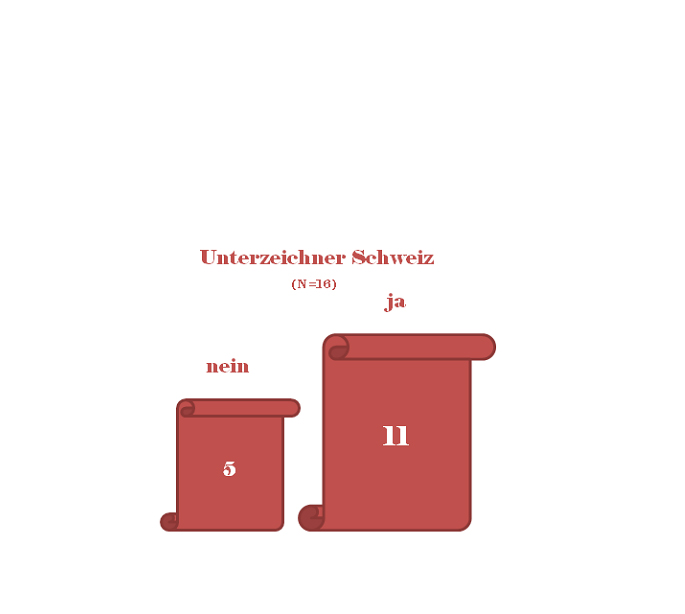
\includegraphics{img/unterzeichner-schweiz.jpg}
\caption{Schweiz - Unterzeichner der Berliner Erklärung}
\end{figure}

In der Schweiz unterzeichneten die wichtigsten
Wissenschaftsorganisationen 2006 die Erklärung.\footnote{Open Access an
  der Universität Basel.
  \url{http://www.ub.unibas.ch/ub-hauptbibliothek/dienstleistungen/publizieren/open-access/},
  25.10.2015.} Zehn Jahre später sind es 21 Schweizer
Unterzeichner.\footnote{Signatoren der Berliner Erklärung:
  \url{http://openaccess.mpg.de/3883/Signatories}, 10.01.2016.} Laut dem
Census gehörten 2014 elf von 16 im Zensus vertretenen Institutionen oder
Schirmorganisationen zu den Signatoren.

Es gibt mit der \emph{ETH E-Collection} der ETH Zürich nur ein
Repositorium (von dem eine Angabe zum \enquote{Launch Date} verfügbar
war), das vor der Berliner Erklärung online ging. Alle anderen OAR
entstanden danach. Um von einer direkten Folge sprechen zu können, gibt
es nicht genügend Anhaltspunkte, aber es ist durchaus möglich, dass die
Open-Access-Aktivitäten nach der Veröffentlichung der Berliner Erklärung
einige Institutionen zur Gründung eines OAR bewegen konnten.

In Österreich unterzeichneten drei von fünf OAR die Berliner Erklärung.
Dies entspricht einer Mehrheit, jedoch bedeutet es auch, dass zwei
Institutionen noch nicht unterzeichnet haben. Insgesamt haben laut der
Signatorenliste der Max-Planck-Gesellschaft mittlerweile neun
österreichische Institutionen die Berliner Erklärung
unterschrieben.\footnote{Signatoren der Berliner Erklärung:
  \url{http://openaccess.mpg.de/3883/Signatories}, 10.01.2016.}

\section*{8 Fakten aus der
Online-Umfrage}\label{fakten-aus-der-online-umfrage}

\paragraph{8.1 Schweiz}\label{schweiz-3}

Die folgenden Auswertungen basieren auf der Online-Umfrage, die Teil des
Census war und weitere Daten über die OAR liefert. Da die Umfrage nicht
von allen Repositorien beantwortet wurde, zeigt sie nur einen Ausschnitt
des Gesamtbildes.

Neun von 16 Schweizer Repositorien beantworten die Umfrage. Davon sind
acht OAR an Universitäten und nur der zhb-dokumentenserver der Zentral-
und Hochschulbibliothek Luzern ist als Repositorium einer
außeruniversitären Forschungseinrichtung vertreten.

Bei allen Fragen wurde zwar ein freies Feld für zusätzliche
\enquote{andere} Antworten zur Verfügung gestellt, jedoch kann dieses
aufgrund der in ihm enthaltenen vertraulichen Information nicht
veröffentlicht werden.

\textbf{\emph{Persistent-Identifier-Systeme }}

In der Umfrage wurde nach dem Einsatz von Persistent-Identifier-Systemen
(PI-Systeme) für die Vergabe von eindeutigen und dauerhaften
Identifikatoren für Open-Access-Voll\-texte gefragt.\footnote{Persistent
  Identifier:
  \url{https://wiki.dnb.de/display/NESTOR/Persistent+Identifier},
  25.10.2015.} In der Schweiz nutzen zwei OAR kein PI-System, während
sieben eines verwenden. Mit fünf Verwendungen ist das
Digital-Object-Identifier-System (DOI) am häufigsten. URNs werden in
zwei Repositorien genutzt, wobei der Dokumentenserver der Universität
Basel DOIs und URNs gleichzeitig nutzt. In Deutschland verhält es sich
umgekehrt. Mit 83\%\footnote{Diese und folgende Prozentzahlen zu den
  Fakten aus der Online-Umfrage aus: Vierkant, Paul: 7 Fakten über
  Deutsche Open-Access-Repositorien:
  \url{https://zenodo.org/record/13045/files/7-Fakten-ueber-Deutsche-Open-Access-Repositorien.svg},
  25.10.2015.} ist der URN in Deutschland bei weitem am meisten
verbreitet, während DOI von 14\% der OAR verwendet wird.

Die ebenfalls zur Auswahl stehenden Systeme Handle und PURL wurden in
der Schweiz im Fall von Handle gar nicht und im Fall von PURL einmal im
OAR \emph{Infoscience} der Ecole Polytechnique Fédérale Lausanne
verwendet. In Deutschland haben diese beiden Systeme mit vier (Handle)
und sechs (PURL) Prozent Verwendung ebenfalls geringere Bedeutung.

\textbf{\emph{Dateiformate zur Langzeitarchivierung }}

Weiterhin wurde nach dem Dateiformat für die Langzeitarchivierung der
Dokumente gefragt. Zur Auswahl standen PDF/A und XML sowie
\enquote{keine} oder \enquote{andere} Formate. Nur vier OAR machten
dahingehende Angaben. Fünf OAR mehr als die Hälfte keine Angaben zu
speziellen Formaten machen. Bei den anderen vier OAR ist das
PDF/A-Format ähnlich wie in Deutschland mit 47\% am meisten verbreitet
und wird durch drei der vier Repositorien verwendet. Zwei OAR nutzen
mehrere Formate. Das \emph{Archive ouverte UNIGE} der Universität in
Genf nutzt sowohl PDF/A als auch XML und das OAR für Digitalisierte
Zeitschriften SEALS nutzt XML sowie ein nicht näher spezifiziertes
\enquote{anderes} Format.

\textbf{\emph{Autorenidentifikatoren}}

Vier OAR nutzen keinerlei Autorenidentifikatoren für die Beschreibung
von Open-Access-Voll\-texten. ORCID und die Personen Normdatei (PND)
werden jeweils einmal verwendet. Alle weiteren OAR nutzen meist interne
Identifikatoren, die in der nicht näher spezifizierten Kategorie
\enquote{Andere} zusammengefasst wurden. In Deutschland nutzt eine
Mehrheit keine IDs und 10\% ebenfalls \enquote{andere} Identifikatoren,
was darauf hindeutet, dass sich bislang sowohl in der Schweiz als auch
in Deutschland kein System für Autorenidentifikatoren durchsetzen
konnte. Weitere 10\% nutzen in Deutschland die PND, die in der Schweiz
nur von einem Repositorium verwendet wird.

\begin{figure}[htbp]
\centering
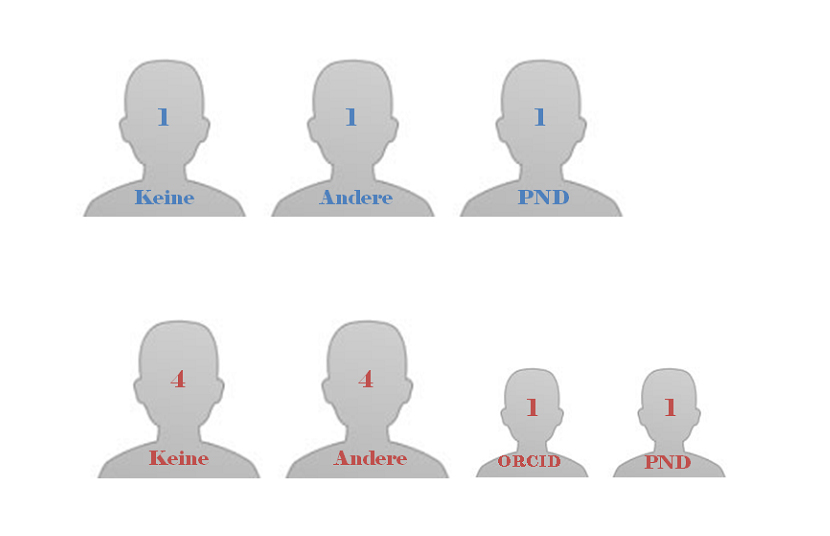
\includegraphics{img/abb9_autorenidentifikatoren.jpg}
\caption{Schweiz - Nutzung von Autorenidentifikatoren
(N=9)}
\end{figure}

\paragraph{8.2 Österreich}\label{uxf6sterreich-3}

Im Falle der OAR Österreichs ist die geringe Teilnahme an der
Online-Umfrage besonders gravierend, da insgesamt nur fünf Repositorien
verzeichnet sind und davon wiederum nur drei den Fragebogen ausgefüllt
haben und im Folgenden berücksichtigt werden können. Dies ist zwar eine
Mehrheit, aber trotzdem eine sehr geringe Menge. Der Vollständigkeit
halber wurden die Analysen dennoch durchgeführt.

Unter den teilnehmenden OAR befinden sich die Repositorien der
Universität Wien, der Wirtschaftsuniversität Wien sowie der
außeruniversitären Forschungseinrichtung Österreichische Akademie der
Wissenschaften.

\textbf{\emph{Persistent-Identifier-Systeme}}

Alle drei OAR nutzen PI-Systeme. Es wird jedoch eventuell ein
Unterschied zwischen Universitäten und außeruniversitären
Forschungseinrichtung sichtbar. Die Universitäten nutzen
\enquote{andere}, nicht namentlich gelistete PI-Systeme, während die
außeruniversitäre Forschungseinrichtung DOIs benennt.

\textbf{\emph{Dateiformate zur Langzeitarchivierung }}

Alle drei Repositorien nutzen Dateiformate zur Langzeitarchivierung,
wobei PDF/A, XML und \enquote{andere} gleichermaßen genutzt werden.

\textbf{\emph{Autorenidentifikatoren}}

\begin{figure}[htbp]
\centering
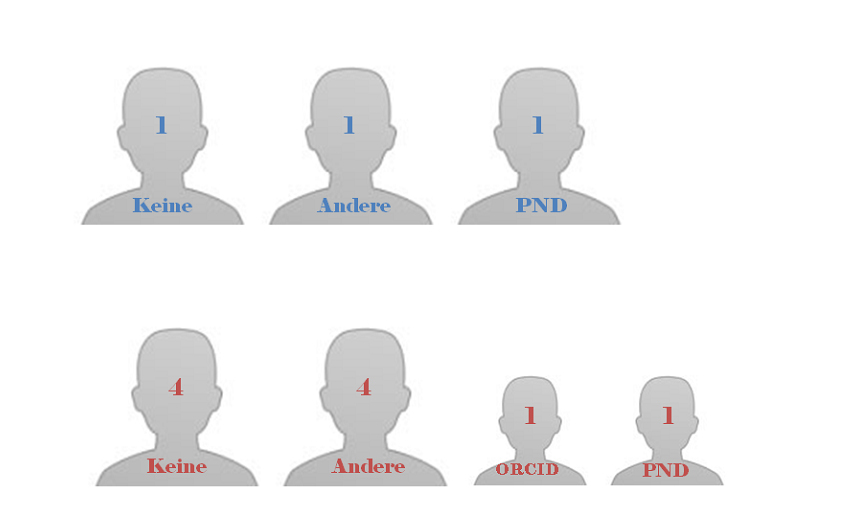
\includegraphics{img/abb10_autorenidentifikatior.jpg}
\caption{Österreich - Nutzung von Autorenidentifikatoren
(N=3)}
\end{figure}

Das Repositorium der Wirtschaftsuniversität Wien nutzt keinerlei
Autorenidentifikatoren. Die anderen beiden OAR verwenden entweder die
PND oder \enquote{andere}. Alle weiteren Identifikatoren finden in den
befragten Repositorien keine Verwendung.

\paragraph{9 Vergleich mit dem Open Access Repository Ranking
2015**}\label{vergleich-mit-dem-open-access-repository-ranking-2015}

Schon 2014 wurde ausgehend von den Daten des Census 2014 das Open Access
Repository Ranking erstellt und im Jahr 2015 auf Basis
weiterentwickelter Kriterien und aktualisierter Daten
veröffentlicht.\footnote{\url{http://repositoryranking.org/}}

Anhand des aktuellen Rankings 2015 stellte sich die Situation im
Vergleich zu 2014 nur leicht verändert dar. Mittlerweile sind sieben
österreichische und 14 Schweizer Repositorien im Ranking vertreten, die
auch den Bedingungen des Census entsprechen würden. In Österreich kamen
mit \emph{Unipub} der Universität Graz und der \emph{Digitalen
Bibliothek} der Universität Innsbruck zwei neue OAR hinzu, die auch
außerhalb des Bundeslandes Wien angesiedelt sind. In der Schweiz
wiederum fehlten 2015 drei Repositorien, die 2014 noch im Census
auftraten, während ein Neues hinzu kam. Nicht mehr im Ranking sind das
\emph{Reproducible Research Repository} der Ecole Polytechnique Fédérale
de Lausanne und die \emph{Digitalisierten Zeitschriften (SEALS)}. Neu
hinzugekommen ist \emph{PHIQ} der Pädagogischen Hochschule St.Gallen.

Im Jahr 2015 gibt es im Vergleich zu den Werten des vorherigen Jahres
rund 211.000 Items weniger in allen 14 verzeichneten OAR der Schweiz.
Das ist auf den allgemeinen Rückgang der OAR-Anzahl zurückzuführen,
während die 10.720 Items Zuwachs in den österreichischen OAR
hauptsächlich durch die neuen OAR zu erklären sind.

Auf die drei Alpenländer gesehen, ist Deutschland weiterhin führend.
Österreich stieg mit dem Repositorium \emph{ePubWU} der
Wirtschaftsuniversität Wien auf Rang 34 ein und die Schweiz auf Rang 27
mit \emph{ZORA} der University of Zurich, während Deutschland alle davor
liegenden Plätze belegt. Damit ist das Repositorium an der Universität
Zürich, welches schon im Census 2014 als das mit der höchsten
Metadatenqualität nach dem DINI-Validator eingeschätzt werden konnte,
das erfolgreichste nicht-deutsche OAR.

Im Ranking 2015 wurde wie im Census ein Umfrageanteil eingebaut, der
hier kurz mit den Ergebnissen der Census Kriterien aus dem Jahr zuvor
verglichen wird. Wieder haben nicht alle OAR alle Fragen beantwortet,
was berücksichtigt werden muss, wenn man sich die Zahlen zu diesen
Kriterien ansehen möchte. In Österreich haben drei der sieben OAR alle
Angaben gemacht. In der Schweiz waren es sechs von 14. Es kann also
sein, dass einige OAR tatsächlich die relevanten Dateiformate oder
Identifikatoren nutzen, dies jedoch nicht angegeben haben, sodass sie in
dieser Auswertung als Nicht-Verwender auftauchen.

Dateiformate für die Langzeitarchivierung wurden laut OARR in Österreich
2015 von keinem OAR verwendet, was allerdings auf der Angabe nur dreier
Repositorien basiert. Im Jahr 2014 nutzten gemäß des Census noch alle
drei an der Umfrage teilnehmenden Repositorien solche Formate. In der
Schweiz nutzte 2015 mit der ETH Zürich ein einziges von 14 OAR
Dateiformate für die Langzeitarchivierung. Im Census 2014 waren es noch
vier von neun Teilnehmenden.

Bei den Angaben bezüglich Persistent Identifier ist davon auszugehen,
dass die Daten aus dem Ranking für Österreich vollständig sind, da alle
OAR angeben PI zu verwenden. Nicht alle weisen auf ihren Webseiten aus
welche verwendet werden. Die drei OAR, die es tun, nutzen jeweils URN,
Handle oder DOI. Auch 2014 nutzten alle drei an der Umfrage
teilnehmenden OAR Identifier, die auf einmal DOI und zweimal
\enquote{andere} PI-Systeme verteilt waren.

Die Situation in der Schweiz stellt sich 2015 ähnlich dar. Bis auf die
Universität St.Gallen nutzen alle Repositorien PI. Die 10 OAR, auf deren
Webseiten dir PI ersichtlich waren, verwendeten DOI. Im Jahr 2014
nutzten alle bis auf zwei PI, wobei ebenfalls am häufigsten auf DOI
zurückgegriffen wurde.

In Österreich ist nur bei drei Repositorien sicher, dass sie 2015 keine
Autorenidentifikatoren nutzten. Die anderen vier haben keine
vollständigen Angaben gemacht, weisen aber in der Kategorie ebenfalls
eine 0 auf. Im Jahr davor nutzte noch eines von drei Repositorien
Autorenidentifikatoren. Für die Schweiz ist im Ranking verzeichnet, dass
keines der 14 OAR, bis auf das der Universität Genf,
Autorenidentifikatoren verwendet. Im Census 2014 lag die Zahl der OAR,
die Autorenidentifikatoren verwenden, noch bei fünf.

\section*{10 Fazit}\label{fazit}

Die Analyse der Daten des Census 2014 erbrachte einige interessante
Ergebnisse. Zunächst ist festzuhalten, dass in beiden Ländern
verhältnismäßig wenige der Definition des Census entsprechende
Open-Access-Repositorien betrieben werden, die Eingang in die
Untersuchung fanden. Während aus Deutschland 152 OAR verzeichnet sind,
sind es aus der Schweiz 16 und aus Österreich gerade einmal fünf für den
Census 2014 relevante OAR. Darüber hinaus finden sich in Österreich nur
in Wien als einzigem der neun Bundesländer überhaupt Repositorien,
während sich in der Schweiz in immerhin acht von 26 Kantonen ein OAR
finden lässt. In Deutschland war nur in Mecklenburg-Vorpommern zum
Zeitpunkt der Erhebung kein Repositorium zu ermitteln, das die Kriterien
für die Aufnahme in den Census 2014 erfüllte.

Ungleich verteilt sind die OAR auch auf die Institutionstypen
Universität, Fachhochschule und außeruniversitäre
Forschungseinrichtungen und Andere. Fachhochschulen gibt es in der
Schweiz eine, die ein OAR betreibt und in Österreich keine.
Außeruniversitäre Forschungseinrichtungen sind in beiden Ländern etwas
breiter vertreten, aber die Mehrheit der Repositorien verteilt sich auf
Universitäten. In Österreich haben trotzdem nur knapp ein Sechstel der
Universitäten ein OAR. In der Schweiz ist es ein Großteil der
universitären Hochschulen. Die Situation in Deutschland sieht ähnlich
aus. Auch dort betreiben hauptsächlich Universitäten OAR.

\begin{figure}[htbp]
\centering
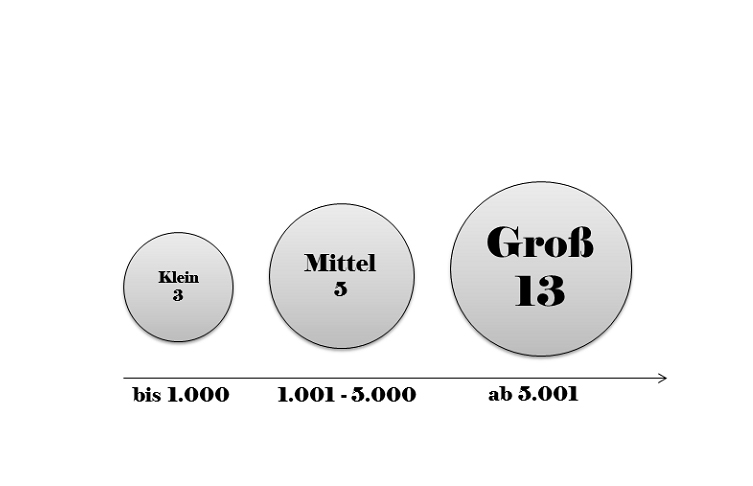
\includegraphics{img/abb11_groesse_repos_at_ch.jpg}
\caption{Größenwerte der OAR in Österreich und der
Schweiz}
\end{figure}

Im Vergleich zu Deutschland gibt es in den Alpenstaaten zwar insgesamt
relativ wenige OAR, dafür halten sie größtenteils viele Items vor und
können als groß klassifiziert werden. Es gibt in beiden Ländern
zusammengenommen nur drei kleine OAR mit bis zu 1.000 Items. Den Rest
machen fünf mittlere und 13 große mit über 5.001 Items aus. Auch hier
ist der Vergleich zu Deutschland interessant, da dort zwar mehr OAR
vorhanden sind, eine knappe Mehrzahl dieser allerdings als klein
eingestuft werden kann. Besonders groß sind die Repositorien der
außeruniversitären Forschungseinrichtungen.\\
Die Metadatenqualität der OAR ist in beiden Ländern eher als gering
einzustufen. Mithilfe des DINI-Validators wurde die Konformität eines
OAR mit den Vorgaben für Metadatenauslieferung gemäß des
DINI-Zertifikats von 2010 überprüft. Die meisten Repositorien in
Österreich und der Schweiz sind im Mittelfeld angesiedelt. Von den 100
möglichen Punkten wurden in Österreich im Durchschnitt 43,64 und in der
Schweiz 54 Punkte erreicht, während in Deutschland dreimal die
Höchstpunktzahl erreicht werden konnte und der Durchschnitt bei 77,5
Punkten liegt.

Bei der Software setzen die Alpenstaaten hauptsächlich auf EPrints. Die
\enquote{Berliner Erklärung über offenen Zugang zu wissenschaftlichem
Wissen} von 2003 gilt als wichtiger Meilenstein in der Entwicklung von
Open Access und wurde in Österreich und der Schweiz jeweils von einer
Mehrheit der befragten die OAR betreibenden Institutionen unterzeichnet.
Insgesamt sind es in beiden Ländern 14 von 21. In Deutschland folgte auf
die Erklärung eine regelrechte Gründungswelle. Auch in Österreich und
der Schweiz kann man beobachten, dass die meisten der im Census 2014
verzeichneten OAR erst nach der Veröffentlichung der Berliner Erklärung
gegründet wurden.

Auf adäquate Datenformate für die Langzeitarchivierung wird in
Österreich in jedem OAR Wert gelegt, wobei die Zahl der in die
Untersuchung einbezogenen OAR wie bereits erläutert gering ist. In der
Schweiz hingegen gibt die Hälfte der OAR an, keine für die
Langzeitarchivierung geeigneten Dateiformate zu verwenden. In
Deutschland verwendet die Mehrheit der Repositorien entsprechende
Dateiformate. Auch dort ist, wie in der Schweiz, das meistverwendete
Format PDF/A.

Zusammengefasst lassen sich die Haupterkenntnisse der Auswertung des
Census 2014 folgendermaßen formulieren:

\begin{itemize}
\item
  Österreich und die Schweiz haben wenige, aber dafür große OAR.
\item
  Die meisten OAR verteilen sich auf Universitäten und außeruniversitäre
  Forschungseinrichtungen. OAR an Fachhochschulen gibt es kaum.
\item
  Die Konformität der Metadatenauslieferung über das OAI-PMH-Protokoll
  ist gemessen der Validierung mit dem DINI-Validator in beiden Ländern
  gering. Hier muss jedoch beachtet werden, dass die Vergabe des
  DINI-Zertifikats für Repositorien aus den Alpenstaaten bislang nicht
  erfolgte.
\item
  Die Software-Lösung EPrints dominiert die OAR-Szene der Alpenstaaten.
\end{itemize}

%autor
\begin{center}\rule{0.5\linewidth}{\linethickness}\end{center}

\textbf{Tabea Bader} (badertab@cms.hu-berlin.de) hat den Bachelor in
Bibliotheks- und Informationswissenschaft und Skandinavistik und
Nordeuropastudien an der Humboldt-Universität zu Berlin abgeschlossen
und studiert jetzt im Master weiter im Bibliotheksbereich.

\end{document}